Včetně elektrické srdeční aktivity, která byla diskutována v minulé sekci a je
hlavní zkoumanou proměnnou, se mezi další periferní biosignály zkoumané v této
práci řadí také elektrodermální a respirační aktivita. V následující podkapitole
jsou tyto periferní biosignály uvedeny do souvislosti s problematikou práce a
předchozími kapitolami. Dále je stručný přehled jak lze zkoumané signály
zaznamenat a zpracovat.

O elektrodermální aktivitě lze hovořit jako o fyziologickém procesu, úzce
spojeném s aktivitou potních žláz v kůži, jež je ovlivňován \gls{ANS}. Aktivita
potních žláz vede ke změnám elektrického odporu kůže. Zvýšením této aktivity tak
dochází k poklesu elektrického odporu kůže (zvýšení kožní vodivosti) a
naopak~\cite{Boucsein2012,Critchley2002,Tronstad2022}. Fredrikson et
al.~\cite{Fredrikson1998} ukázali, že EDA je úzce spojená s aktivitou cingulární
kůry, sekundární zrakové kůry a pravé inferiorní parietální kůry, přičemž
nejsilnější korelace byla pozorována v pravé insulární kůře, která je součástí
\gls{CAN}. Další studie naznačují mnohočetné souvislosti mezi změnami kožní
vodivosti a \gls{CAN} regiony~\cite{Critchley2002,Buchwald2019,Caruelle2019,Sanchez2020}.
EDA tedy nachází velké uplatnění v neuropsychofyziologickém výzkumu ale stejně jako u HRV
se zde vyskytují problémy s interpretací metrik, které z ní
vycházejí~\cite{Blechert2016}. Z anatomického, fyziologického a biofyzikálního
hlediska byla již elektrodermální aktivita důkladně rozebrána v~\cite{Boucsein2012}.
Úzkou provázanost kožní vodivosti a kognitivní zátěže s využitím EDA pro její detekci
a hodnocení podkládají studie~\cite{Bahauddin2021,Ghaderyan2018,Hossain2019,
    Nourbakhsh2012,Paas2003,Posada2018,Shi2007,Shimomura2008}.

Respirační aktivitou se rozumí proces dýchání, při kterém dochází k výměně
kyslíku a oxidu uhličitého mezi plícemi a okolím. Dýchací ústrojí bylo již
důkladně popsáno v~\cite{Kara2010}. Respirační signál jako takový odráží
cyklické změny objemu plic během dýchání. Dýchací aktivita je ovlivněna celou
řadou faktorů, včetně fyzické aktivity, stresu, emocí a i kognitivních nároků.
Například kognitivní úkoly vyžadující trvalou pozornost nebo vyšší nároky na
pracovní paměť mohou zvýšit dechovou námahu a spotřebu kyslíku v mozku. Obecně
se amplituda a frekvence dechového signálu zvyšuje s rostoucí kognitivní
zátěží~\cite{Ayres2021}. Existuje mnoho studií, které vypovídají o významném
vztahu mezi respiračním signálem a \gls{CL}, avšak oproti srdeční a
elektrodermální aktivitě je tento signál mnohem častěji zanedbáván. To může
vysvětlovat větší počet protichůdných a negativních studií, které popírají
význam RSP při detekci a hodnocení kognitivní
zátěže~\cite{Ayres2021,Grassmann2016}.

\subsection{Měření biosignálů}
\label{subsec:srdecni_aktivita}
V následujících sekcích jsou popsany principy měření a postupy zpracování
periferních biosignálu, které byly využívány pro účely této diplomové práce.
Těmi jsou konkrétně srdeční, elektrodermální a respirační aktivita.

\subsubsection{Elektrická srdeční aktivita}
Záznam elektrické srdeční aktivity (elektrokardiogram) je výstupem komplexních
fyziologických a technologických procesů. Z fyziologického hlediska je třeba
nahlédnout na celulární úroveň, kde díky toku iontů přes buněčné membrány a mezi
sousedními buňkami vznikají transmembránové iontové proudy. Geneze těchto proudů
je synchronizována díky srdečnímu cyklu, během kterého dochází k tvorbě časově
závislého elektrické pole v myokardu. Toto elektrické pole pak podléhá
interferenci různých dalších struktur, jako jsou plíce, krev a kosterní svalstvo
až kůže. Na kůži jsou poté proudy detekovány elektrodami umístěnými na určitých
místech končetin a trupu v takové konfiguraci, aby vytvářely svody, konkrétně
bipolární svody~\cite{mirvis2001}. Elektrofyziologie myokardu byla již detailně
popsána v~\cite{Goldberger2017,Cihak2016,Stejfa2006,Weinhaus2005}.

Svody zaznamenávají rozdíl potenciálů mezi dvěma elektrodami, přičemž jedna je
označována jako kladná a druhá záporná. Bipolární potenciál se následně získává
jako rozdíl potenciálů kladné a záporné elektrody. U některých konfigurací je
elektricky spojeno více elektrod, které představují záporný člen bipolárního
páru, označovaný jako referenční elektroda. Výstupní potenciály elektrod jsou ve
finále zesíleny, filtrovány~\cite{Goldberger2017,mirvis2001}.

Jednou z konfigurací je standardní klinické EKG, které zahrnuje záznamy z 12
svodů. Svody v tomto případě sestávají ze standardních končetinových svodů
(svody I, II a III), šesti prekordiálních svodů (svody V1 až V6) a ze tří
rozšířených (augmentovaných) končetinových svodů\footnote{Prekordiální a
    rozšířené končetinové elektrody jsou často označované jako \enquote{unipolární}
    svody.} (svody aVR, aVL a aVF)~\cite{Goldberger2017,mirvis2001}.

\begin{figure}[htb!]
    \begin{center}
        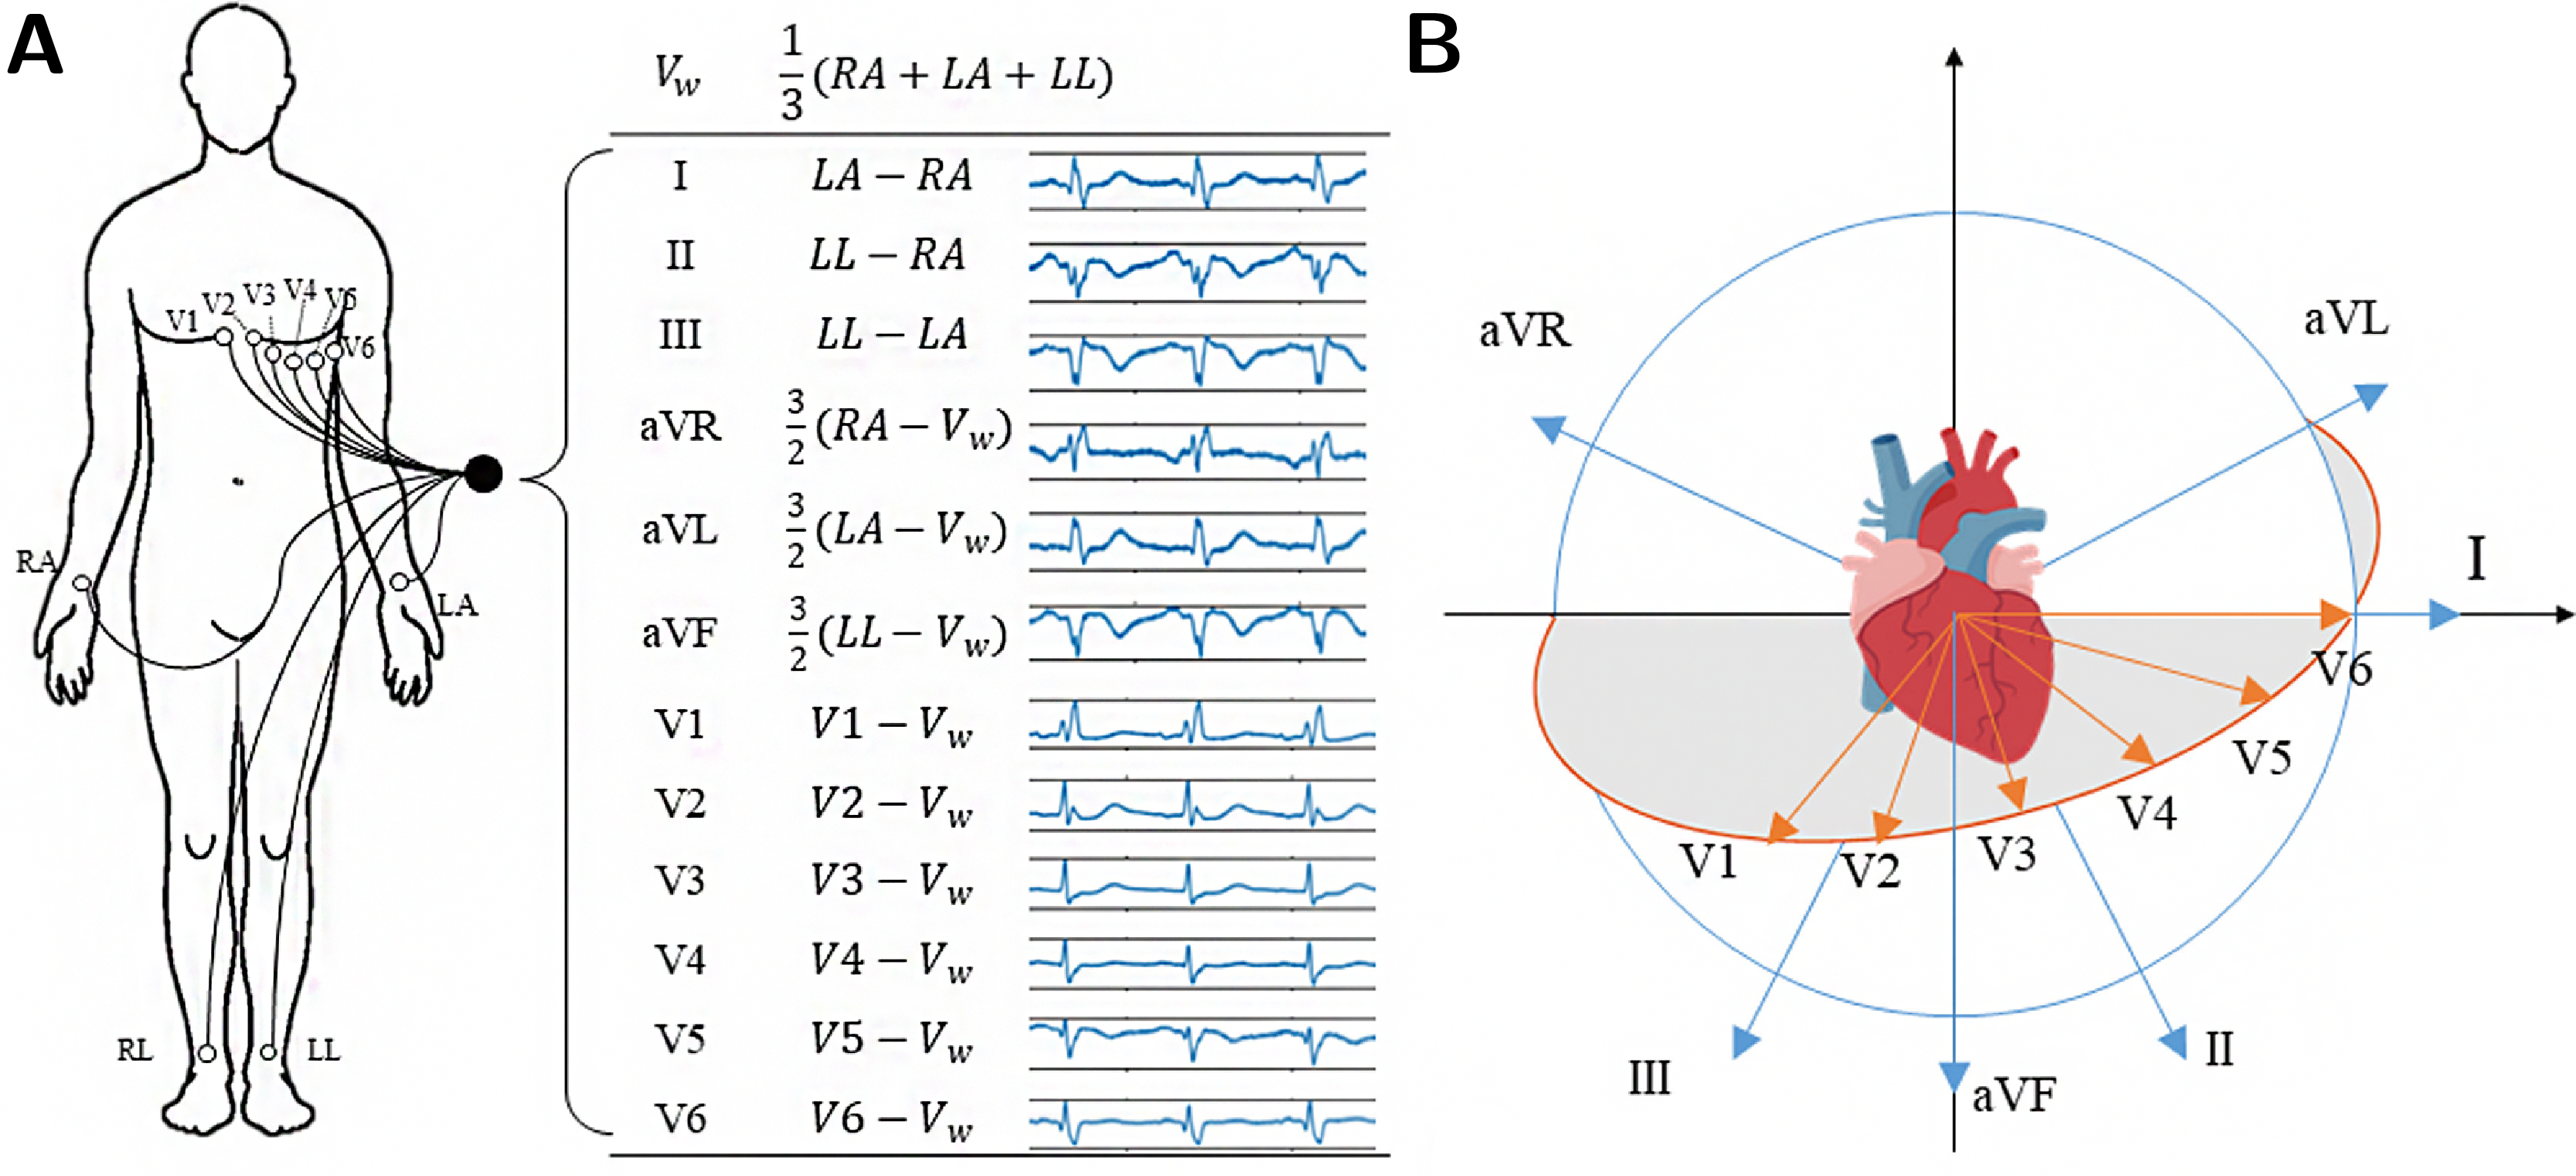
\includegraphics[width=1\linewidth]{figures/ecg_leads}
        \caption{Ilustrace 12svodového EKG systému. \textbf{A)} Prostorové
            rozmístění 10 elektrod: tři končetinové svody, tři rozšířené končetinové
            svody a šest prekordiálních (hrudních) svodů, které byly vytvořeny mezi
            fyzickými elektrodami a virtuální elektrodou známou jako Wilsonův
            centrální terminál ($V_W$). \textbf{B)} Rozdíly elektrických potenciálů
            mezi elektrodami odrážejí elektrickou aktivitu srdce z různých
            prostorových úhlů~(Přeloženo a převzato z~\cite{Yao2020})}
        \label{fig:ecg_leads}
    \end{center}
\end{figure}

\paragraph{Standardní končetinové svody.}
Standardní končetinové svody zachycují rozdíly potenciálů mezi dvěma
končetinami. Elektroda na pravé noze slouží jako referenční, snižuje šum a není
tak součástí konfigurace svodů. Svody jsou uspořádány do trojúhelníku, který se
často nazývá jako Einthovenův trojúhelník. Toto uspořádání zajišťuje, že
potenciál snímaný ve svodu II odpovídá součtu potenciálů měřených ve svodech I a
III~\cite{Goldberger2017,mirvis2001}.

\paragraph{Prekordiální svody a wilsonův centrální terminál.}
Prekordiální svody se používají k záznamu potenciálu v každém ze šesti určených
míst trupu vzhledem k referenci. Na každé místo se umístí aktivní elektroda
připojená ke kladnému vstupu záznamového systému. Referenčním vstupem je složená
elektroda známá jako Wilsonova centrální svorka, která je vytvořena kombinací
výstupu elektrod levé paže (LA), pravé paže (RA) a levé nohy (LL)
prostřednictvím odporů (5000~\si{\ohm})~\cite{Goldberger2017,mirvis2001}.

\paragraph{Rozšířené končetinové svody.}
Jak již bylo zmíněno, třemi augmentovanými svody jsou aVR, aVL a aVF. U svodu
aVR je aktivní elektrodou sloužící jako pozitivní vstup elektroda pravé paže,
zatímco u svodu aVL je to elektroda levé paže a u svodu aVF elektroda levé nohy.
Referenční potenciál je zde vytvořen spojením dvou končetinových elektrod, které
se nepoužívají jako aktivní. Účelem tohoto modifikovaného referenčního systému
je generovat signál s vyšší amplitudou než při použití Wilsonovy centrální
svorky jako referenční elektrody~\cite{Goldberger2017,mirvis2001}.

\paragraph{Další svodové systémy.}
Byly vyvinuty různé svodové systémy, které umožňují detekovat diagnosticky
významné informace, jež nemusí být zachyceny standardním 12svodovým EKG, a
zlepšit efektivitu záznamu, přenosu a ukládání EKG. Používají se například levé
zadní svody k detekci akutních posterolaterálních infarktů nebo elektrodová pole
o 80 nebo více elektrodách k zobrazení potenciálů povrchu těla jako izopotenciálních
map~\cite{Goldberger2017,mirvis2001}. Přehled dalších svodových systému včetně
nositelných byl popsán v~\cite{Baig2013,Majumder2018,Serhani2020}.

\subsubsection{Elektrodermální aktivita}
V úvodu kapitoly bylo řečeno, že princip měření EDA je založen na skutečnosti,
že činnost potních žláz v kůži, která je regulována sympatickým nervovým
systémem, vede ke změnám vodivosti kůže. Díky tomu, a jak může vyplývat z
minulých kapitol, je měření EDA běžně používanou metodou pro hodnocení
fyziologických reakcí souvisejících s emočními a kognitivními procesy.

\begin{figure}[htb!]
    \begin{center}
        \includegraphics[width=1\linewidth]{figures/EDA}
        \caption{\textbf{A)} Možná místa měření kožní vodivosti. \textbf{B)}
            Typická odezva elektrodermální aktivity~(Upraveno a převzato
            z~\cite{Janssen2012,Vavrinsky2021})}
        \label{fig:eda_mereni}
    \end{center}
\end{figure}

Měření elektrodermální aktivity zahrnuje umístění dvou elektrod na kůži, přičemž
jedna měří rozdíly potenciálů mezi dvěma body na kůži a druhá slouží jako
referenční elektroda. Elektrody se obvykle umísťují na prsty nebo dlaň ruky, i
když lze použít i jiná místa, například chodidla nebo čelo (viz
Obr.~\ref{fig:eda_mereni}A) a měří se elektrická vodivost kůže v reakci na malý
stejnosměrný nebo střídavý proud proud~\cite{Caruelle2019,Boucsein2012}.

Z pohledu způsobu měření elektrodermální aktivity lze tedy rozlišovat dvě hlavní
kategorie: endosomatická a exosomatická měření. V rámci endosomatického měření
se zaznamenává pouze potenciál generovaný kůží bez použití vnějšího zdroje. U
exosomatického měření se využívají externí zdroje, jako je právě střídavý nebo
stejnosměrný proud přiváděný na kůži. Aplikace konstantního stejnosměrného
napětí nebo proudu umožňuje měření vodivosti kůže (resp. odporu kůže podle
Ohmova zákona). Pokud se ale aplikuje konstantní střídavé napětí nebo proud, tak
lze měřit kožní admitanci (resp. kožní impedanci). Nejpoužívanější metodou pro
exosomatická měření je metoda stejnosměrného konstantního napětí, a to primárně
díky jednoduššímu procesu vyhodnocování a interpretace než je tomu tak u
endosomatického způsobu~\cite{Boucsein2012,Li2022,Posada2020,Caruelle2019}.

Měřená kožní vodivost nebo kožní potenciál se vyjadřují v jednotkách vodivosti
(mikrosiemens, \si{\micro\siemens}) a napětí (\si{\milli\volt}). V naměřeném
signálu se odrážejí změny v různých časových škálách, které se běžně dělí na dvě
složky: tonickou (\gls{SCL}) a fázickou (\gls{SCR}). Tonická složka představuje
velikost kožní vodivosti nebo potenciálu v nepřítomnosti sudomotorické nervové
aktivity\footnote{Sudomotorická nervová aktivita se vztahuje k \gls{ANS}
    kontrole aktivity potních žláz v reakci na různé environmentální a individuální
    faktory.}, zatímco ta fázická se týká rychlých změn kožní vodivosti nebo
potenciálu jako přímého důsledku sudomotorického vzruchu. Fázická složka je
charakterizován nástupem (SCR ris.), dobou nárůstu (SCR ris. t.), amplitudou
(SCR amp.) a dobou zotavení (SCR rec. tc.). Na Obr.~\ref{fig:eda_mereni} lze
vidět průběh EDA složek společně s jejich korespondujícím popisem. Tonické a
fázické složky lze oddělit pomocí technik zpracování
signálu~\cite{Boucsein2012,Li2022,Posada2020,Caruelle2019,Caruelle2019}.

\subsubsection{Respirační aktivita}
\label{subsec:respiracni_aktivita}
Pro měření dechové aktivity (resp. dechové frekvence) je k dispozici mnoho
metod, od přímého měření ventilace až po nepřímé měření pohybů souvisejících s
dýcháním. V této sekci je stručný přehled často používaných metod měření dechové
aktivity.

\begin{figure}[htb!]
    \begin{center}
        \includegraphics[width=1\linewidth]{figures/rsp_measure}
        \caption{Různé technologie pro měření dechové frekvence ($f_R$). Nahoře
        z kategorie snímačů proudění vzduchu, kde $ΔP(Q)$ je změna úbytku tlaku
        způsobená prouděním vzduchu $Q$. Uprostřed z kategorie snímačů teploty,
        kde $R(T)$ je změna odporu způsobená vlivem teploty $T$. Dole z
        kategorie tenzometrických snímačů, kde $f(\mathcal{E})$ je změna odporu
        způsobená deformačním tlakem $\mathcal{E}$. $V(X)$ je výstupní
        napětí~(Upraveno a převzato z~\cite{Massaroni2019})}
        \label{fig:rsp_mereni}
    \end{center}
\end{figure}

Jednou z nejběžnějších metod měření dechové aktivity je přímé měření ventilace.
Ventilace je celkový objem vzduchu, který se během každého nádechu přesune do
plic a z plic ven, a lze ji měřit pomocí několika technik včetně spirometrie,
pletysmografie, a kapnometrie. Spirometrie měří objem vzduchu, který je
vdechován a vydechován, zatímco pletysmografie měří změny tlaku v uzavřené
komoře během dýchání. Kapnometrie měří koncentraci oxidu uhličitého ve
vydechovaném vzduchu, což úzce souvisí s ventilací. Tyto techniky umožňují
přesné měření dechové aktivity, ale mohou být invazivní a vyžadují
specializované vybavení~\cite{Massaroni2019,Massaroni2021,Liu2019}. 

Alternativní metodou měření dechové aktivity je nepřímé měření pohybů
souvisejících s dýcháním. Tyto pohyby lze detekovat pomocí senzorů umístěných na
hrudníku nebo břiše, jako jsou piezoelektrické senzory, tenzometry nebo
akcelerometry. Tyto snímače detekují změny tvaru nebo pohybu hrudníku nebo
břicha během dýchání a lze je použít k odhadu dechové frekvence a objemu. Tyto
metody jsou méně invazivní než přímé měření ventilace a lze je použít v reálném
prostředí, avšak u některých populací nebo za určitých podmínek mohou být méně
přesné~\cite{Massaroni2019,Massaroni2021,Fazio2021,Liu2019}.

Další nově se objevující metodou měření dechové aktivity je používání
nositelných zařízení, jako jsou chytré hodinky, které mohou detekovat změny
dechových vzorců pomocí fotopletysmografie nebo akcelerometrie.
Fotopletysmografie měří změny objemu krve pomocí světelných senzorů, zatímco
akcelerometrie měří pohyb pomocí pohybových senzorů. Tyto metody jsou
neinvazivní a lze je použít v přirozeném prostředí s tím, že mohou být omezené
ve své přesnosti a preciznosti~\cite{Massaroni2019,Massaroni2021,Fazio2021,
Leube2020,Liu2019,Nam2022,Zschocke2022}. 

\subsection{Postupy zpracování biosignálů}
\label{subsec:postupy_zpracovani_biosignalu}
Zpracování biosignálů označuje techniky a postupy používané k získání informací
z biosignálů, ke zvýšení jejich kvality a k interpretaci jejich významu. V této
sekci je uveden přehled hlavních postupů zpracování biosignálů, včetně jejich
akvizice, předzpracování, extrakce příznaků a klasifikace. 

V návaznosti na předchozí sekci, sběr signálu znamená tedy proces záznamu
biosignálů z lidského těla pomocí měřicích zařízení, jako jsou senzory nebo
elektrody. Kvalita zaznamenaných signálů závisí na různých faktorech, jako je
typ a umístění snímačů, odstup signálu od šumu a vzorkovací frekvence. Například
signály EKG se zaznamenávají pomocí elektrod a jejich umístění ovlivňuje kvalitu
zaznamenaných signálů, protože různé oblasti srdce mohou mít různou sílu nebo
frekvenci signálu. Kromě toho se odstup signálu od šumu týká poměru žádoucího
signálu a nežádoucího šumu v zaznamenaných signálech. Čím vyšší je poměr
signál/šum, tím jsou zaznamenané signály jasnější a spolehlivější. A konečně
vzorkovací frekvence označuje frekvenci, s jakou jsou signály vzorkovány nebo
digitalizovány. Čím vyšší je vzorkovací frekvence, tím přesnější je digitální
reprezentace signálů~\cite{Escabi2005,Karagiannis2011}.

\begin{figure}[htb!]
    \begin{center}
        \includegraphics[width=1\linewidth]{figures/signal_processing_diagram}
        \caption{Řetězec procesů od získání biomedicínského signálu po fázi
        analýzy~(Přeloženo a převzato z~\cite{Karagiannis2011})}
        \label{fig:zpracovani_biosignalu_diagram}
    \end{center}
\end{figure}

Předzpracování se týká postupů používaných k přípravě zaznamenaných signálů pro
další analýzu. Mezi postupy předzpracování patří především filtrování signálu.
Žádoucí je často navržení takového filtru, který rovnou koriguje kolísání nulové
izolinie a potlačuje nežádoucí artefakty (síťový šum, svalové artefakty, apod.).
V některých případech však nestačí pouze frekvenčně selektivní filtrace a volí
se jiné přístupy. Zvolený přístup závisí na zdroji a charakteru signálu.
Porovnání metod předzpracování srdeční, elektrodermální a respirační aktivity
bylo vypracováno v ~\cite{Escabi2005,Khodadad2018,Power2020,Subramanian2019}. 

Extrakce příznaků označuje postupy používané k extrakci relevantních informací
nebo charakteristik z předzpracovaných signálů. Extrakce příznaků je důležitým
krokem při zpracování biosignálů, protože jednak snižuje dimenzionalitu signálů
a také zvýrazňuje právě relevantní informace. Z biosignálů lze extrahovat různé
typy příznaků, například z časové, z frekvenční nebo nelineární
oblasti~\cite{Escabi2005,Karagiannis2011}. Krishnan a Athavale popsali trendy v
extrakci příznaků biomedicínských signálů v~\cite{Krishnan2018}.

Klasifikací se rozumí postupy používané k přiřazení značky (anotace) nebo
kategorie biosignálu na základě jeho extrahovaných vlastností (příznaků).
Klasifikace je dalším důležitým krokem při zpracování biosignálů, protože
umožňuje identifikovat vzory nebo trendy v signálech a předpovídat fyziologický
stav nebo kondici subjektu~\cite{Escabi2005,Karagiannis2011}. Možnosti využití
klasifikace (resp. metod strojového učení) pro biomedicínské aplikace byly
popsány v~\cite{Foster2014,Kording2018,Strzelecki2022}.

Zpracování biosignálů se potýká s různými problémy a omezeními, jako je
variabilita signálů, složitost postupů zpracování a interpretace výsledků.
Variabilitou signálů je myšleno, že biosignály se mohou lišit od subjektu k
subjektu, od sezení k sezení nebo dokonce v rámci jednoho sezení. Tato
variabilita může ovlivnit kvalitu a spolehlivost zaznamenaných signálů a může
vyžadovat použití sofistikovanějších metod předzpracování a
klasifikaci~\cite{Escabi2005,Karagiannis2011}.